\documentclass[12pt, a4paper]{article}
% \usepackage{ctex}
\usepackage[margin=1in]{geometry} 
\usepackage{amsmath,amsthm,amssymb}
\usepackage{bm}
\usepackage{cases}
\usepackage{graphicx}
\usepackage{hyperref}
\hypersetup{hidelinks}
\usepackage{amsfonts}
\usepackage{authblk}
\newcommand{\E}{\mathbb{E}}
\newcommand{\R}{\mathbb{R}}
\title{PRML Note\\C02 Probability Distributions}
\author{Yang Zhao}
\affil{Department of Automation, Tsinghua University}
\date{}

\begin{document}
    \maketitle
    \begin{itemize}
        \item Given a finite set $x_1,x_2,\cdots,x_N$ of observation, which is i.i.d, modeling
        the probability distribution $p(x)$ of a random variable $x$, which is called density
        estimation, is ill-posed.
        \item \textit{conjugate prior}: leads to posterior distributions having the same 
        functional form as the prior.
        \item \textit{parametric approach}: must assume the specific functional form for the 
        distribution.(Limitation)
        \item \textit{non-parametric approach}: 1.depends on size of the data set. 2.still has 
        parameters, which control the model complexxity rather than the form of the distribution
    \end{itemize}
    %
    %  Chapter 1 Binary Variables
    %
    \section{Binary Variables}
    \begin{itemize}
        \item $x\in\{0,1\}$, let $0\le\mu\le 1$ we have
        \begin{align*}
            &p(x=1|\mu)=\mu\\
            &p(x=0|\mu)=1-\mu
        \end{align*}
        \textit{The Bernoulli distribution}
        \begin{align*}
            Bern(x|\mu)&=\mu^x(1-\mu)^{1-x}\\
            \E \lbrack x\rbrack&=\mu\\
            var\lbrack x\rbrack&=\mu(1-\mu)
        \end{align*}
        \item a data set $D=\{x_1,x_2,\cdots,x_N\}$
        \begin{align*}
            p(D|\mu)&=\prod_{n=1}^Np(x_n|\mu)=\prod_{n=1}^N\mu^{x_n}(1-\mu)^{1-x_n}\\
            lnp(D|\mu)&=\sum_{n=1}^N\{x_nln\mu+(1-x_n)ln(1-\mu)\}
        \end{align*}
        Let 
        \[\frac{\partial{lnp(D|\mu)}}{\partial{\mu}}=0\]
        we have
        \[
            \mu_{ML}=\frac{m}{N}
            \]
        where $m$ is the number of observations of $x=1$ within this data.
        \item \textit{binomial distribution}
        \begin{align*}
            Bin(m|N,\mu)&=C_N^m\mu^m(1-\mu)^{N-m} \\
            \E \lbrack m\rbrack&=N\mu\\
            var\lbrack m\rbrack&=N\mu(1-\mu)
        \end{align*}
        Using the result that for independent variables $x$ and $z$, $\E\lbrack x+z
        \rbrack=\E x+\E z$ and $var\lbrack x+z\rbrack=varx+varz$, we can easily
        get the expectation and variance.
        \item \textit{beta distribution}
        \begin{align}
            \label{BetaDistribution}
            Beta(\mu|a,b)&=\frac{\Gamma(a+b)}{\Gamma(a)\Gamma(b)}\mu^{a-1}(1-\mu)
            ^{b-1}\\
            \E\lbrack\mu\rbrack&=\frac{a}{a+b}\nonumber\\
            var\lbrack\mu\rbrack&=\frac{ab}{(a+b)^2(a+b+1)}\nonumber
        \end{align}
        where
        \begin{equation*}
            \Gamma(x)=\int_0^\infty \mu^{x-1}e^xdx
        \end{equation*}
        and
        \begin{equation*}
            \int_0^1Beta(\mu|a,b)d\mu=1
        \end{equation*}
        The parameters $a$ and $b$ are called \textit{hyperparameters}
        \item posterior distribution
        \begin{align*}
            p(\mu|m,N,a,b)&\propto p(\mu|a,b)p(m|N,\mu)\\
            &\propto \mu^{m+a-1}(1-\mu)^{N-m+b-1}\\
        \end{align*}
        where $l=N-m$. Comparing with the equation \ref{BetaDistribution}, we have
        \begin{equation*}
            p(\mu|m,l,a,b)=\frac{\Gamma(m+l+a+b)}{\Gamma(m+a)\Gamma(l+b)}
            \mu^{m+a-1}(1-\mu)^{l+b-1}
        \end{equation*}
        in which the parameters $a,b$ is the effective number of observations that
        need not be integers.
        \item \textit{Sequential approach}: make use of observations once at a time, 
        or in small batches, then discard them before the next observations.
        \begin{enumerate}
            \item independent of the choice of prior and of likelihood function
            \item depends only on the assumption of i.i.d data
        \end{enumerate}
        This method is used in
        \begin{enumerate}
            \item real-time learning scenarios
            \item large data sets
            \item maximum likelihood methods can also be cast into a sequential 
            framework.
        \end{enumerate}
        \item Given observed data set $D$, to predict $x$
        \begin{align*}
            p(x=1|D)=&\int_0^1p(x=1|\mu)p(\mu|D)d\mu\\
            =&\int_0^1\mu p(\mu|D)d\mu\\
            =&\E\lbrack \mu|D\rbrack\\
            =&\frac{m+a}{m+a+l+b}
        \end{align*}
        \item A general property of Bayesian learning: As observing more and more 
        data, the uncertainly represented by the posterior distribution will steadily 
        decrease.
        \item The Bayesian and maximum likelihood results will agree in the limit of 
        an infinitely large data set.\\
        For a finite data set: posterior mean for $\mu$ always lies between the prior 
        mean and the maximum likelihood estimate for $\mu$.
        \item Consider a general Bayesian inference problem for a parameter $\theta$, 
        observed a data set $D$, the joint distribution $p(\theta,D)$. We have the
        following result
        \begin{align}
            \label{Eq:Expectation}
            \E_\theta\lbrack\theta\rbrack&=\E_D\lbrack\E_\theta\lbrack\theta|D\rbrack
            \rbrack\\
            \label{Eq:Variance}
            var_\theta\lbrack\theta\rbrack&=\E_D\lbrack var_\theta\lbrack\theta|D
            \rbrack\rbrack+var_D\lbrack\E_\theta\lbrack\theta|D\rbrack\rbrack
        \end{align}
        The process to get the equation \ref{Eq:Expectation} and \ref{Eq:Variance} is 
        below:
        \begin{align*}
            \E_y\lbrack\E_x\lbrack x|y\rbrack\rbrack&=\int(\int xp(x|y)dx)p(y)dy\\
            &=\iint xp(x|y)p(y)dxdy\\
            &=\iint xp(x,y)dxdy\\
            &=\int x(\int p(x,y)dy)dx\\
            &=\int xp(x)dx\\
            &=\E\lbrack x\rbrack
        \end{align*}
        which is equal to the equation \ref{Eq:Expectation}. Let
        \begin{align*}
            a(y)=&\int xp(x|y)dx=\E\lbrack x|y\rbrack\\
            b(y)=&\int x^2p(x|y)dx=\E\lbrack x^2|y\rbrack\\
            E=&\E_y\lbrack\E_x\lbrack x|y\rbrack\rbrack=\E\lbrack x\rbrack
        \end{align*}
        Thus,
        \begin{align}
            \label{Eq:ConditionalVariance}
            var_x\lbrack x|y\rbrack&=\E\lbrack x^2|y\rbrack-(\E\lbrack x|y\rbrack)^2
            \nonumber\\
            &=b(y)-a^2(y)
        \end{align}
        So
        \begin{align}
            \label{eq:ExpectationVariance}
            \E_y\lbrack var_x\lbrack x|y\rbrack\rbrack&=\int(b(y)-a^2(y))p(y)dy\\
            \label{eq:VarianceExpectation}
            var_y\lbrack\E_x\lbrack x|y\rbrack\rbrack&=
            \E\big((\E_x(x|y)-\E_y\E_x(x|y))^2\big)\nonumber\\
            &=\int(a(y)-E)^2p(y)dy
        \end{align}
        Add the equation \ref{eq:ExpectationVariance} and \ref{eq:VarianceExpectation},
        we have
        \begin{align*}
            &\E_y\lbrack var_x\lbrack x|y\rbrack\rbrack+var_y\lbrack\E_x\lbrack x|y
            \rbrack\rbrack\\
            &=\int(b(y)-a^2(y))p(y)dy+\int(a(y)-E)^2p(y)dy\\
            &=\int\lbrack(a(y)-E)^2+(b(y)-a^2(y))\rbrack p(y)dy\\
            &=\int\lbrack E^2+b(y)-2Ea(y)\rbrack p(y)dy\\
            &=E^2\int p(y)dy+\int b(y)p(y)dy-2E\int a(y)p(y)dy\\
            &=E^2+\E x^2-2E^2\\
            &=\E x^2-E^2\\
            &=var\lbrack x\rbrack
        \end{align*}
    \end{itemize}
    %
    %  Chapter 2 Multinomial Variables
    %
    \section{Multinomial Variables}
    \begin{itemize}
        \item 1-of-K scheme $\bm{x}=(0,0,\cdots,1,\cdots,0,0)^T$\\
        denote the probability of $x_k=1$ by the parameter $\mu_k$, then the 
        distribution of $\bm{x}$ is given
        \begin{equation}
            p(\bm{x}|\bm{\mu})=\prod_{k=1}^K\mu_k^{x_k}
        \end{equation}
        where $\bm{\mu}=(\mu_1,\mu_2,\cdots,\mu_K)^T$, $\mu_k\ge 0$ and 
        $\sum_k\mu_k=1$. This distribution can be regarded as a generalization of 
        the Bernoulli distribution to more than two outcomes.
        \begin{align*}
            \sum_xp(\bm{x}|\bm{\mu})&=\sum_{k=1}^K\mu_k=1\\
            \E\lbrack\bm{x}|\bm{\mu}\rbrack&=\bm{\mu}
        \end{align*}
        \item Consider a data set $D$ of $N$ independent observations 
        $\bm{x}_1,\bm{x}_2,\cdots,\bm{x}_N$, the corresponding likelihood function
        takes the form
        \begin{equation*}
            p(D|\mu)=\prod_{n=1}^N\prod_{k=1}^K\mu_k^{x_{nk}}=\prod_{k=1}^K\mu_k^
            {\sum_n x_{nk}}=\prod_{k=1}^K\mu_k^{m_k}
        \end{equation*}
        where $m_k=\sum_n x_{nk}$, which represent the number of observations of 
        $x_k=1$. And the maximum likelihood solution is below:
        \begin{equation*}
            \mu_k^{ML}=\frac{m_k}{N}
        \end{equation*}
        \item \textit{Multinomial distribution}
        \begin{equation*}
            Mult(m_1,m_2,\cdots,m_k|\bm{\mu},N)=\frac{N!}{m_1!m_2!\cdots m_k!}
            \prod_{k=1}^K\mu_k^{m_k}
        \end{equation*}
        where $\sum_{k=1}^Km_k=N$.
        \item \textit{Dirichlet distribution}
        \begin{equation*}
            Dir(\bm{\mu}|\bm{\alpha})=\frac{\Gamma(\alpha_0)}{\Gamma(\alpha_1)\cdots
            \Gamma(\alpha_K)}\prod_{k=1}^K\mu_k^{\alpha_k-1}
        \end{equation*}
        where $\bm{\alpha}=(\alpha_1,\cdots,\alpha_K)^T$ and $\alpha_0=\sum_{k=1}^K
        \alpha_k$.
        \item posterior distribution
        \begin{align*}
            p(\bm{\mu}|D,\bm{\alpha})&\propto p(D|\bm{\mu})p(\bm{\mu}|\bm{\alpha})
            \propto \prod_{k=1}^K\mu_k^{\alpha_k+m_k-1}\\
            &=Dir(\bm{\mu}|\bm{\alpha}+\bm{m})\\
            &=\frac{\Gamma(\alpha_0+N)}{\Gamma(\alpha_1+m_1)\cdots
            \Gamma(\alpha_K+m_K)}\prod_{k=1}^K\mu_k^{\alpha_k+m_k-1}
        \end{align*}
    \end{itemize}
    %
    %  Chapter 3 The Gaussian Distribution
    %
    \section{The Gaussian Distribution}
    \begin{itemize}
        \item \textit{The Gaussian Distribution}
        \begin{align}
            \mathcal{N}(x|\mu,\sigma^2)&=\frac{1}{(2\pi\sigma^2)^{1/2}}e^{-\frac{(x-\mu)^2}
            {2\sigma^2}}\\
            \mathcal{N}(\bm{x}|\bm{\mu},\bm{\Sigma})&=\frac{1}{(2\pi)^{D/2}}\frac{1}{\vert
            \bm{\Sigma}\vert^{1/2}}e^{-\frac{1}{2}(\bm{x}-\bm{\mu})^T\bm{\Sigma}^{-1}
            (\bm{x}-\bm{\mu})}
        \end{align}
        \item For the univariate Gaussian distribution, we have obtain below propositions
        at Chapter 1
        \begin{align*}
            \int\mathcal{N}(x|\mu,\sigma^2)dx&=1\\
            \int\mathcal{N}(x|\mu,\sigma^2)xdx&=\mu\\
            \int\mathcal{N}(x|\mu,\sigma^2)x^2dx&=\mu^2+\sigma^2
        \end{align*}
        \item \textit{quadratic form}
        \begin{equation*}
            \Delta^2=(\bm{x}-\bm{\mu})^T\bm{\Sigma}^{-1}(\bm{x}-\bm{\mu})
        \end{equation*}
        which is called \textit{Mahalanobis distance} from $\bm{\mu}$ to $\bm{x}$
        \item Without loss of generality, we can assume the matrix $\bm{\Sigma}$ to be 
        symmetric. To prove this, we assume the matrix $\bm{\Sigma}$ is non-symmetric, 
        we have
        \begin{align*}
            \bm{x}^T\bm{\Sigma}\bm{x}&=\bm{x}^T(\frac{\bm{\Sigma}+\bm{\Sigma}^T}{2}+
            \frac{\bm{\Sigma}-\bm{\Sigma}^T}{2})\bm{x}\\
            &=\bm{x}^T(\frac{\bm{\Sigma}+\bm{\Sigma}^T}{2})\bm{x}
        \end{align*}
        where $(\bm{\Sigma}+\bm{\Sigma}^T)/2$ is symmetric.
        \item For $\bm{\Sigma}$ is a real, symmetric matrix, let $\bm{U}=(\bm{u}_1,
        \bm{u}_2,\cdots,\bm{u}_D)$ be an orthonormal matrix, i.e. $\bm{U}\bm{U}^T=\bm{I}$, 
        we have
        \begin{align}
            \label{eq:desMatrix}
            \bm{\Sigma}&=\bm{U}diag(\lambda_1,\lambda_2,\cdots,\lambda_D)\bm{U}^T\nonumber\\
            &=(\bm{u}_1,\bm{u}_2,\cdots,\bm{u}_D)\begin{pmatrix}
                \lambda_1 & && \\
                &\lambda_2&&\\
                 & & \ddots&\\
                && & \lambda_D
            \end{pmatrix}\begin{pmatrix}
                \bm{u}_1^T\\
                \bm{u}_2^T\\
                \vdots\\
                \bm{u}_D^T
            \end{pmatrix}
        \end{align}
        where $\lambda_k$ is the eigenvalue of $\bm{\Sigma}$ and $\bm{u}_k$ is the 
        corresponding eigenvector. And the equation \ref{eq:desMatrix} can be rewritten
        as below
        \begin{equation}
            \bm{\Sigma}=\sum_{i=1}^D\lambda_i\bm{u}_i\bm{u}_i^T
        \end{equation}
        and
        \begin{equation}
            \bm{\Sigma}^{-1}=\sum_{i=1}^D\frac{1}{\lambda_i}\bm{u}_i\bm{u}_i^T
        \end{equation}
        if we define that $\bm{y}=\bm{U}^T(\bm{x}-\bm{\mu})$ and $\bm{y}=(y_1,y_2,\cdots,y_D)^T$,
        we have
        \begin{equation}
            \Delta^2=\sum_{i=1}^{D}\frac{y_i^2}{\lambda_i}
        \end{equation}
        \item For the Gaussian distribution to be well defined, it is necessary for all of 
        eigenvalues $\lambda_i$ of the covariance matrix to be strictly positive, otherwise the 
        distribution cannot be properly normalized.
        \item from $x$ to $y$, the Jacobian matrix $J$ with elements given by
        \begin{equation*}
            \bm{J}_{ij}=\frac{\partial{x_i}}{\partial{y_j}}=\bm{U}_{ji}
        \end{equation*}
        So $|\bm{J}|=1$ and $|\Sigma|^{1/2}=\prod_{j=1}^D\lambda_j^{1/2}$
        Thus in the $y$ coordinate system, the Gaussian distribution takes the form
        \begin{equation}
            p(\bm{y})=p(\bm{x})|\bm{J}|=\prod_{j=1}^D\frac{e^{-y_j^2/2\lambda_j}}{(2\pi\lambda_j)
            ^{1/2}}
        \end{equation}
        \item For the multivariate Gaussian distribution, we have
        \begin{align}
            \label{eq:NormGaussian}
            \int\mathcal{N}(\bm{x}|\bm{\mu},\bm{\Sigma})d\bm{x}&=1\\
            \label{eq:MeanGaussian}
            \mathbb{E}(\bm{x})=\int\mathcal{N}(\bm{x}|\bm{\mu},\bm{\Sigma})\bm{x}d\bm{x}
            &=\bm{\mu}\\
            \label{eq:VarGaussian}
            \mathbb{E}(\bm{x}\bm{x}^T)=\int\mathcal{N}(\bm{x}|\bm{\mu},\bm{\Sigma})
            \bm{x}\bm{x}^Td\bm{x}&=\bm{\mu}\bm{\mu}^T+\bm{\Sigma}
        \end{align}
        \item To prove equation \ref{eq:NormGaussian}
        \begin{align*}
            \int\mathcal{N}(\bm{x}|\bm{\mu},\bm{\Sigma})d\bm{x}&=\int p(\bm{y})d\bm{y}\\
            &=\prod_{j=1}^D\int\frac{e^{-y_j^2/2\lambda_j}}{(2\pi\lambda_j)^{1/2}}dy_j\\
            &=1
        \end{align*}
        which is $D$ production of univariate Gaussian distribution.
        \item To prove equation \ref{eq:MeanGaussian}
        \begin{align*}
            \mathbb{E}(x)&=\frac{1}{(2\pi)^{D/2}}\frac{1}{\vert
            \bm{\Sigma}\vert^{1/2}}\int e^{-\frac{1}{2}(\bm{x}-\bm{\mu})^T\bm{\Sigma}^{-1}
            (\bm{x}-\bm{\mu})}\bm{x}d\bm{x}\\
            &=\frac{1}{(2\pi)^{D/2}}\frac{1}{\vert\bm{\Sigma}\vert^{1/2}}\int e^{-\frac{1}{2}
            \bm{z}^T\bm{\Sigma}^{-1}\bm{z}}(\bm{z}+\bm{\mu})d\bm{z}\\
        \end{align*}
        Obviously, $e^{-\frac{1}{2}\bm{z}^T\bm{\Sigma}^{-1}\bm{z}}$ is an even function, which
        means
        \begin{equation}
            \label{even}
            \int e^{-\frac{1}{2}\bm{z}^T\bm{\Sigma}^{-1}\bm{z}}\bm{z}d\bm{z}=0
        \end{equation}
        Thus
        \begin{equation}
            \mathbb{E}(x)=\frac{1}{(2\pi)^{D/2}}\frac{1}{\vert\bm{\Sigma}\vert^{1/2}}\bm{\mu}
            \int e^{-\frac{1}{2}\bm{z}^T\bm{\Sigma}^{-1}\bm{z}}d\bm{z}=\bm{\mu}
        \end{equation}
        \item To prove equation \ref{eq:VarGaussian}
        \begin{align}
            \mathbb{E}(\bm{x}\bm{x}^T)&=\frac{1}{(2\pi)^{D/2}}\frac{1}{\vert
            \bm{\Sigma}\vert^{1/2}}\int e^{-\frac{1}{2}(\bm{x}-\bm{\mu})^T\bm{\Sigma}^{-1}
            (\bm{x}-\bm{\mu})}\bm{x}\bm{x}^Td\bm{x}\nonumber\\
            &=\frac{1}{(2\pi)^{D/2}}\frac{1}{\vert\bm{\Sigma}\vert^{1/2}}\int e^{-\frac{1}{2}
            \bm{z}^T\bm{\Sigma}^{-1}\bm{z}}(\bm{z}+\bm{\mu})(\bm{z}+\bm{\mu})^Td\bm{z}\nonumber\\
            &=\frac{1}{(2\pi)^{D/2}}\frac{1}{\vert\bm{\Sigma}\vert^{1/2}}\int e^{-\frac{1}{2}
            \bm{z}^T\bm{\Sigma}^{-1}\bm{z}}(\bm{z}\bm{z}^T+\bm{z}\bm{\mu}^T+\bm{z}^T\bm{\mu}+
            \bm{\mu}\bm{\mu}^T)d\bm{z}\nonumber\\
            &=\bm{\mu}\bm{\mu}^T+\frac{1}{(2\pi)^{D/2}}\frac{1}{\vert\bm{\Sigma}\vert^{1/2}}\int 
            e^{-\frac{1}{2}\bm{z}^T\bm{\Sigma}^{-1}\bm{z}}\bm{z}\bm{z}^Td\bm{z}
        \end{align}
        where using equation \ref{even} to eliminate the cross-terms $\bm{\mu}\bm{z}^T$ and 
        $\bm{z}\bm{\mu}^T$. The method we introduce below is really important. 
        Because $\bm{y}=\bm{U}^T(\bm{x}-\bm{\mu})=\bm{U}^T\bm{z}$, we get
        $\bm{z}=\bm{U}\bm{y}=\sum_{j=1}^Dy_j\bm{u}_j$, which gives
        \begin{align*}
            &\frac{1}{(2\pi)^{D/2}}\frac{1}{\vert\bm{\Sigma}\vert^{1/2}}\int 
            e^{-\frac{1}{2}\bm{z}^T\bm{\Sigma}^{-1}\bm{z}}\bm{z}\bm{z}^Td\bm{z}\\
            &=\frac{1}{(2\pi)^{D/2}}\frac{1}{\vert\bm{\Sigma}\vert^{1/2}} \sum_{i=1}^D\sum_{j=1}^D
            \bm{u}_i\bm{u}_j^T\int e^{-\sum_{k=1}^D\frac{y_k^2}{2\lambda_k}}y_iy_jd\bm{y}\\
            &=\sum_{i=1}^D\bm{u}_i\bm{u}_i^T\lambda_i=\bm{\Sigma}
        \end{align*}
        where the integral will vanish by symmetry unless $i=j$, so
        \begin{equation}
            \mathbb{E}(\bm{x}\bm{x}^T)=\bm{\mu}\bm{\mu}^T+\bm{\Sigma}
        \end{equation}
        Thus
        \begin{equation}
            cov\lbrack\bm{x}\rbrack=\mathbb{E}\bm{x}^2-(\mathbb{E}\bm{x})^2=\bm{\Sigma}
        \end{equation}
        \item \textit{significant limitations}
        \begin{enumerate}
            \item number of independent parameters grows quadratically with $D$
            \item we can assume $\bm{\Sigma}$ to be diagonal or to be proportional to the identity 
            matrix. 
            \item Only has a single maximum
        \end{enumerate}
        Thus the Gaussian distribution can be both too flexible in the sense of too many parameters, 
        while also being too limited in the range of distributions that it can adequately represent.
        \begin{figure}[htbp]
            \centering
            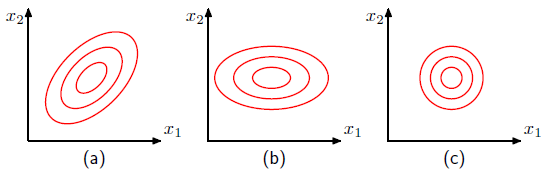
\includegraphics[width=0.9\textwidth]{figures/Figure2_8.png}
            \caption{the covariance matrix of (a) is general form, of (b) is diagonal and
            of (c) is proportiional to the identity matrix}
        \end{figure}
        \item Note that the exponent in a general Gaussian distribution $\mathcal{N}(\bm{x}|\bm{\mu},
        \bm{\Sigma})$ can be written
        \begin{equation*}
            -\frac{1}{2}(\bm{x}-\bm{\mu})^T\bm{\Sigma}^{-1}(\bm{x}-\bm{\mu})=-\frac{1}{2}\bm{x}^T
            \bm{\Sigma}\bm{x}+\bm{x}^T\bm{\Sigma}^{-1}\bm{\mu}+const
        \end{equation*}
        where we can directly get the $\bm{\Sigma}$ and $\bm{\mu}$.
        \item \textit{Conditional Gaussian distribution}\\
        If two sets of variables are joint Gaussian, then the conditional distribution of one 
        set conditioned on the other is again Gaussian.\\
        Consider $\bm{x}\in\R \sim \mathcal{N}(\bm{x}|\bm{\mu},\bm{\Sigma})$ and we partition $\bm{x}$
        into two subsets $\bm{x}_a$ and $\bm{x}_b$, so that $\bm{x}=(\bm{x}_a^T, \bm{x}_b^T)^T$, 
        $\bm{\mu}=(\bm{\mu}_a^T,\bm{\mu}_b^T)^T$ and 
        \begin{equation*}
            \bm{\Sigma}=\begin{pmatrix}
                \bm{\Sigma}_{aa} & \bm{\Sigma}_{ab}\\
                \bm{\Sigma}_{ba} & \bm{\Sigma}_{bb}
            \end{pmatrix}
        \end{equation*}
        We denote the covariance matrix by \textit{precision matrix}
        \begin{equation*}
            \bm{\Lambda} \equiv\bm{\Sigma}^{-1}
        \end{equation*}
        where 
        \begin{equation*}
            \bm{\Lambda}=\begin{pmatrix}
                \bm{\Lambda}_{aa} & \bm{\Lambda}_{ab}\\
                \bm{\Lambda}_{ba} & \bm{\Lambda}_{bb}
            \end{pmatrix}
        \end{equation*}
        Using the equation \ref{Eq:InvOfPartitionedMatrix} we can obtain the result of $\bm{\Lambda}_{aa},
        \bm{\Lambda}_{ab}, \bm{\Lambda}_{ba}, \bm{\Lambda}_{bb}$ and $\bm{\Lambda}_{ab}=\bm{\Lambda}_{ba},
        \bm{\Lambda}_{aa}=\bm{\Lambda}_{aa}^T,\bm{\Lambda}_{bb}=\bm{\Lambda}_{bb}^T$.
         So we obtain
        \begin{align*}
            -\frac{1}{2}(\bm{x}-\bm{\mu})^T\bm{\Sigma}^{-1}(\bm{x}-\bm{\mu})&=-\frac{1}{2}
            (\bm{x}_a-\bm{\mu}_a)^T\bm{\Lambda}_{aa}(\bm{x}_a-\bm{\mu}_a)-
            (\bm{x}_a-\bm{\mu}_a)^T\bm{\Lambda}_{ab}(\bm{x}_b-\bm{\mu}_b)\\
            &-\frac{1}{2}(\bm{x}_b-\bm{\mu}_b)^T\bm{\Lambda}_{bb}(\bm{x}_b-\bm{\mu}_b)\\
            &=-\frac{1}{2}\bm{x}_a^T\bm{\Lambda}_{aa}\bm{x}_a+\bm{x}_a^T(\bm{\Lambda}_{aa}\bm{\mu}_a-
            \bm{\Lambda}_{ab}(\bm{x}_b-\bm{\mu}_b))+const
        \end{align*}
        Thus
        \begin{align}
            \bm{\Sigma}_{a\vert b}&=\bm{\Lambda}_{aa}^{-1}\\
            \bm{\mu}_{a\vert b}&=\bm{\mu}_a-\bm{\Lambda}_{aa}^{-1}\bm{\Lambda}_{ab}(\bm{x}_b-\bm{\mu}_b)
        \end{align}
        or
        \begin{align}
            \bm{\Sigma}_{a\vert b}&=\bm{\Sigma}_{aa}-\bm{\Sigma}_{ab}\bm{\Sigma}_{bb}^{-1}\bm{\Sigma}_{ba}\\
            \bm{\mu}_{a\vert b}&=\bm{\mu}_a+\bm{\Sigma}_{ab}\bm{\Sigma}_{bb}^{-1}(\bm{x}_b-\bm{\mu}_b)
        \end{align}
        Thus
        \begin{equation}
            p(\bm{x}_a|\bm{x}_b)=\mathcal{N}(\bm{x}_a|\bm{\mu}_{a|b},\bm{\Lambda}_{aa}^{-1})
        \end{equation}
        Note that $\bm{\Sigma}_{a\vert b}$ is independent of $\bm{x}_b$ and $\bm{\mu}_{a\vert b}$ is a linear
        function of $\bm{x}_b$. This represents an example of \textit{linear-Gaussian} model.
        \item \textit{Marginal Gaussian distribution}
        \begin{equation}
            p(\bm{x}_a)=\int p(\bm{x}_a,\bm{x}_b)d\bm{x}_b=\mathcal{N}(\bm{x}_a|\bm{\mu}_a,\bm{\Sigma}_{aa})
        \end{equation}
        \begin{figure}[htbp]
            \begin{minipage}[t]{0.45\textwidth}
                \centering
                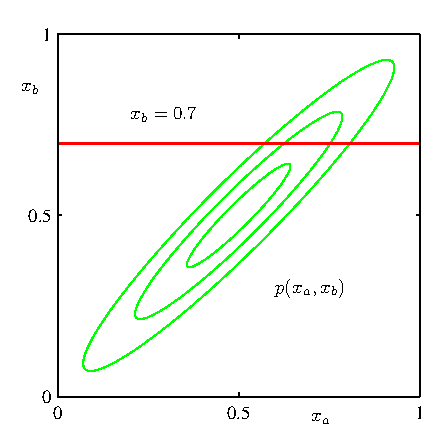
\includegraphics[width=0.9\textwidth]{figures/Figure2_9a.eps}
            \end{minipage}
            \hfill
            \begin{minipage}[t]{0.45\textwidth}
                \centering
                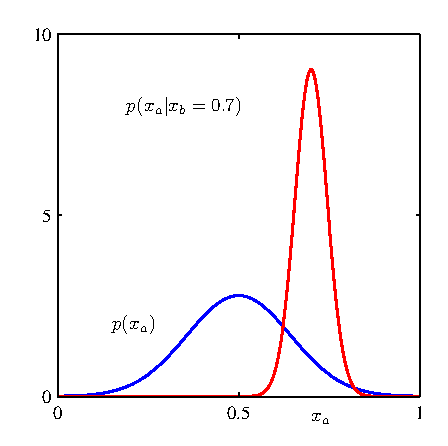
\includegraphics[width=0.9\textwidth]{figures/Figure2_9b.eps}
            \end{minipage}
            \caption{The conditional Gaussian distribution and the marginal Gaussian distribution}
        \end{figure}
        \item Given a marginal Gaussian distribution for $\bm{x}$ and a conditional Gaussian distribution
        for $\bm{y}$ given $\bm{x}$ in the form
        \begin{align*}
            p(\bm{x})&=\mathcal{N}(\bm{x}|\bm{\mu},\bm{\Lambda}^{-1})\\
            p(\bm{y}|\bm{x})&=\mathcal{N}(\bm{y}|\bm{A}\bm{x}+\bm{b},\bm{L}^{-1})
        \end{align*}
        we can easily get 
        \begin{align*}
            p(\bm{y})&=\mathcal{N}(\bm{y}|\bm{A}\bm{\mu}+\bm{b},\bm{L}^{-1}+\bm{A\Lambda}^{-1}
            \bm{A}^T)\\
            p(\bm{x}|\bm{y})&=\mathcal{N}(\bm{x}|\bm{\Sigma}(\bm{A}^T\bm{L}(\bm{y}-\bm{b})+\bm{\Lambda}
            \bm{\mu}),\bm{\Sigma})
        \end{align*}
        where
        \begin{equation*}
            \bm{\Sigma}=(\bm{\Lambda}+\bm{A}^T\bm{LA})^{-1}
        \end{equation*}
        \item Given a data set $\bm{X}=(\bm{x}_1,\bm{x}_2,\cdots,\bm{x}_N)^T$, using the maximum likelihood
        function method, we can obtain
        \begin{align}
            \label{eq:muML}
            \bm{\mu}_{ML}&=\frac{1}{N}\sum_{n=1}^N\bm{x}_n\\
            \bm{\Sigma}_{ML}&=\frac{1}{N}\sum_{n=1}^N(\bm{x}-\bm{\mu}_{ML})(\bm{x}-\bm{\mu}_{ML})^T
        \end{align}
        and if we evalute the expectation of the solution, we can obtain the following results
        \begin{align*}
            \E\lbrack\bm{\mu}_{ML}\rbrack&=\bm{\mu}\\
            \E\lbrack\bm{\Sigma}_{ML}\rbrack&=\frac{N-1}{N}\bm{\Sigma}
        \end{align*}
        So
        \begin{equation*}
            \widetilde{\bm{\Sigma}}=\frac{1}{N-1}\sum_{n=1}^N(\bm{x}-\bm{\mu}_{ML})(\bm{x}-\bm{\mu}_{ML})^T
        \end{equation*}
        \item  Using the equation \ref{eq:muML}, we can rewritten it as below
        \begin{align}
            \label{eq:muMLSeq}
            \bm{\mu}_{ML}^{(N)} &= \frac{1}{N}\sum_{n=1}^N\bm{x}_n\nonumber\\
            &=\frac{1}{N}\bm{x}_N+\frac{1}{N}\sum_{n=1}^{N-1}\bm{x}_n\nonumber\\
            &=\frac{1}{N}\bm{x}_N+\frac{N-1}{N}\bm{\mu}_{ML}^{(N-1)}\nonumber\\
            &=\bm{\mu}_{ML}^{(N-1)}+\frac{1}{N}(\bm{x}_N-\bm{\mu}_{ML}^{(N-1)})
        \end{align}
        However, we will not always be able to derive a sequential algorithm like this, which leads us to
        the \textit{Robbins-Monro algorithm}, which is introduced in Appendix.\\
        By definition, we have
        \begin{equation*}
            -\frac{\partial}{\partial{\theta}}\Big(\frac{1}{N}\sum_{n=1}^Nlnp(\bm{x}_n|\theta)\Big)
            \Big\vert_{\theta_{ML}}=0
        \end{equation*}
        Exchanging the derivative and the summation, taking the limit $N\rightarrow\infty$, we have
        \begin{equation*}
            -lim_{N\rightarrow\infty}\frac{1}{N}\sum_{n=1}^N\frac{\partial}{\partial{\theta}}
            lnp(\bm{x}_N|\theta)=\E_x\Big\lbrack-\frac{\partial}{\partial{\theta}}lnp(\bm{x}|\theta)
            \Big\rbrack
        \end{equation*}
        So we can get
        \begin{equation}
            \theta_N=\theta_{N-1}-a_{N-1}\frac{\partial}{\partial{\theta_{N-1}}}lnp(\bm{x}_N|\theta_{N-1})
        \end{equation}
        which equals to
        \begin{equation*}
            \theta_N=\theta_{N-1}-a_{N-1}\frac{x-\mu_{ML}}{\sigma^2}
        \end{equation*}
        If we choose $a_{N-1}=\sigma^2/N$, we can obtain the equation \ref{eq:muMLSeq}.
        \item We suppose the variance $\sigma^2$ is known and we consider the task of inferring the mean 
        $\mu$ given a set of $N$ observations $\bm{X}=(x_1,x_2,\cdots,x_N)$. The likelihood function is 
        given by
        \begin{equation*}
            p(\bm{X}|\mu)=\frac{1}{(2\pi\sigma^2)^{N/2}}e^{-\frac{1}{2\sigma^2}\sum_{n=1}^N(x_n-\mu)^2}
        \end{equation*}
        If we choose a prior $p(\mu)=\mathcal{N}(\mu|\mu_0,\sigma_0^2)$, the posterior distribution is 
        given by
        \begin{equation*}
            p(\mu|\bm{X})=\mathcal{N}(\mu|\mu_N,\sigma_N^2)\propto p(\bm{X}|\mu)p(\mu)
        \end{equation*}
        where
        \begin{align*}
            \mu_N&=\frac{\sigma^2}{N\sigma_0^2+\sigma^2}\mu_0+\frac{N\sigma_0^2}{N\sigma_0^2+\sigma^2}
            \mu_{ML}\\
            \frac{1}{\sigma_N^2}&=\frac{1}{\sigma_0^2}+\frac{N}{\sigma^2}
        \end{align*}
        which can be easily get by completing the square in the exponent.
        \item \textit{student's t-distribution}
        \begin{equation}
            St(x|\mu,\lambda,\nu)=\frac{\Gamma(\nu/2+1/2)}{\Gamma(\nu/2)}\Big(\frac{\lambda}{\pi\nu}
            \Big)^{1/2}\Big\lbrack 1+\frac{\lambda(x-\mu)^2}{\nu}\Big\rbrack^{-(\nu+1)/2}
        \end{equation}
        where $\mu$ is the mean, the $\lambda$ is sometimes called the precision of t-distribution, 
        the $\nu$ is the degrees of freedom.
        \begin{align*}
            \E (x)&=\mu &if\quad\nu>1\\
            var (x)&=\frac{\nu}{\nu-2}\lambda^{-1} &if\quad\nu>2\\
            mode (x)&=\mu&
        \end{align*}
        Comparing with Gaussian distribution, the student's t-distribution could be more robust for 
        the outliers.
        \begin{figure}[htbp]
            \begin{minipage}[t]{0.45\textwidth}
                \centering
                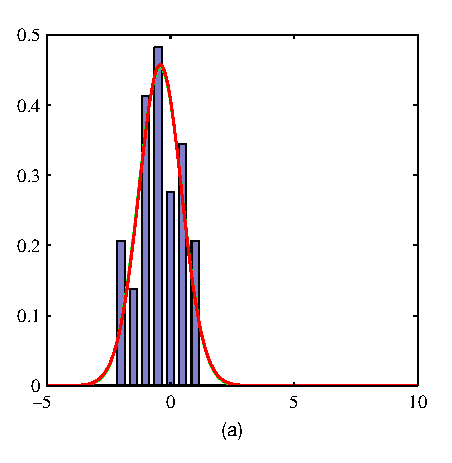
\includegraphics[width=0.9\textwidth]{figures/Figure2_16a.eps}
            \end{minipage}
            \hfill
            \begin{minipage}[t]{0.45\textwidth}
                \centering
                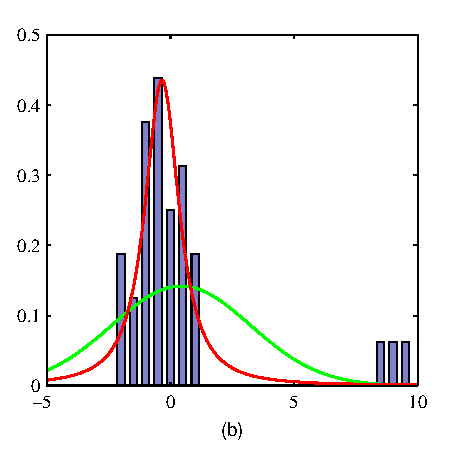
\includegraphics[width=0.9\textwidth]{figures/Figure2_16b.eps}
            \end{minipage}
            \caption{The robustness of t-distribution}
        \end{figure}
    \end{itemize}
    %
    % Chapter 5 The nonparametic methods
    %
    \section{The Nonparametic Methods}
    \begin{itemize}
        \item \textit{histogram methods for density estimation}
        \begin{equation}
            p_i=\frac{n_i}{N\Delta_i}
        \end{equation}
        in which we often have $\Delta_i=\Delta$. $\Delta_i$ is the width of the $i$-th bin, $n_i$ is 
        the number of observations of $x$ falling in the $i$-th bin and $N$ is the total number of 
        observations. The properties of this method is below:
        \begin{enumerate}
            \item Data can be discarded after the histogram has been computed.
            \item If the data are arriving sequentially.
        \end{enumerate}
        And the limitations are below
        \begin{enumerate}
            \item the results is dependent on the choice of edge locations and the width of bins.
            \item the estimated density has discontinuities due to the bin edge.
            \item Cannot be used for high dimensionality because of curse of dimensionality.
        \end{enumerate}
        \item \begin{equation}
            p(x)=\frac{K}{NV}
        \end{equation}
        where $K$ is the number of points lieing inside $\mathcal{R}$ and $V$ is the volume of 
        $\mathcal{R}$. Note that this two parameters are contradictory. We want the $V$ can be 
        enough small but we also want the $K$ is large enough. If we fix the $K$, this method is 
        called \textit{K-nearest-neighbour} and if we fix the $V$, this method is called 
        \textit{kernel approach}.
    \end{itemize}
    %
    % Chapter 6 Appendix
    %
    \section{Appendix}
    \begin{itemize}
        \item \textit{Gamma Function}
        \begin{equation}
            \label{GammaFunction}
            \Gamma(x)=\int_0^\infty u^{x-1}e^{-u}du
        \end{equation}
        At below we prove the relation $\Gamma(x+1)=x\Gamma(x)$
        \begin{align*}
            \Gamma(x+1)&=\int_0^\infty u^xe^{-u}du\\
            &=-u^xe^{-u}\Big\vert_0^\infty+\int_0^\infty xu^{x-1}e^{-u}du\\
            &=0+x\Gamma(x)\\
            &=x\Gamma(x)
        \end{align*}
        \item \textit{The expression of Lagrange Multipliers in constant, vector and matrix}\\
        For the below problem, which is expressed by exercise 2.14
        \begin{align*}
            max\quad &H\lbrack\bm{x}\rbrack=-\int p(\bm{x})lnp(\bm{x})d\bm{x}\\
            s.t.\quad &\int p(\bm{x})d\bm{x}=1\\
            &\int p(\bm{x})\bm{x}d\bm{x}=\bm{\mu}\\
            &\int p(\bm{x})(\bm{x}-\bm{\mu})(\bm{x}-\bm{\mu})^Td\bm{x}=\bm{\Sigma}
        \end{align*}
        where the first constraints is constant, the second constraints is vector and the third 
        constraints is matrix. The Lagrange function of the uppon problem is below
        \begin{align}
            g(\lambda,\bm{m},\bm{L})=H\lbrack\bm{x}\rbrack+\lambda\Big(\int p(\bm{x})d\bm{x}-1
            \Big)+\bm{m}^T\Big(\int p(\bm{x})\bm{x}d\bm{x}-\bm{\mu}\Big)\nonumber\\
            +tr\Big(\bm{L}\big(\int p(\bm{x})(\bm{x}
            -\bm{\mu})(\bm{x}-\bm{\mu})^Td\bm{x}-\bm{\Sigma}\big)\Big)
        \end{align}
        \item \textit{The inverse matrix of a partitioned matrix}
        \begin{equation}
            \label{Eq:InvOfPartitionedMatrix}
            \begin{pmatrix}
                \bm{A} & \bm{B}\\
                \bm{C} & \bm{D}
            \end{pmatrix}^{-1}=\begin{pmatrix}
                \bm{M} & -\bm{MBD}^{-1}\\
                -\bm{D}^{-1}\bm{CM} & \bm{D}^{-1}+\bm{D}^{-1}\bm{CMBD}^{-1}
            \end{pmatrix}
        \end{equation}
        where we have defined
        \begin{equation}
            \label{Eq:SchurComplement}
            \bm{M}=(\bm{A}-\bm{BD}^{-1}\bm{C})^{-1}
        \end{equation}
        which is known as \textit{Schur complement}. The process to get the equation 
        \ref{Eq:InvOfPartitionedMatrix} is below. We denote
        \begin{equation*}
            \begin{pmatrix}
                \bm{A} & \bm{B}\\
                \bm{C} & \bm{D}
            \end{pmatrix}^{-1}=\begin{pmatrix}
                \bm{E} & \bm{F}\\
                \bm{G} & \bm{H}
            \end{pmatrix}
        \end{equation*}
        Thus
        \begin{equation*}
            \begin{pmatrix}
                \bm{A} & \bm{B}\\
                \bm{C} & \bm{D}
            \end{pmatrix}\begin{pmatrix}
                \bm{E} & \bm{F}\\
                \bm{G} & \bm{H}
            \end{pmatrix}=\begin{pmatrix}
                \bm{I_A} & \bm{0}\\
                \bm{0} & \bm{I_D}
            \end{pmatrix}
        \end{equation*}
        which equals to
        \begin{align*}
            &\bm{AE}+\bm{BG}=\bm{I_A}\\
            &\bm{CE}+\bm{DG}=\bm{0}\\
            &\bm{AF}+\bm{BH}=\bm{0}\\
            &\bm{CF}+\bm{DH}=\bm{I_D}
        \end{align*}
        if we assume $\bm{D}$ and $\bm{A}-\bm{BD}^{-1}\bm{C}$ are invertible, solve this 
        linear equation, we can easily  get the equation \ref{Eq:InvOfPartitionedMatrix}. 
        Note that if we assume $\bm{A}$ and $\bm{CA}^{-1}\bm{B}+\bm{D}$ are invertible, the 
        solution will be in different form. In fact, the following conditions are equivalent:
        \begin{enumerate}
            \item the original matrix is invertible.
            \item $\bm{D}$ and $\bm{A}-\bm{BD}^{-1}\bm{C}$ are invertible
            \item $\bm{A}$ and $\bm{CA}^{-1}\bm{B}+\bm{D}$ are invertible
        \end{enumerate}
        which can be proved by $(2)\Rightarrow (1)$, $(3)\Rightarrow (1)$, 
        $(1)\Rightarrow (2)$ and $(1)\Rightarrow (3)$.
        \item \textit{Woodbury matrix identity}
        \begin{eqnarray}
            \label{eq:Woodbury}
            (\bm{A}+\bm{UCV})^{-1}=\bm{A}^{-1}-\bm{A}^{-1}\bm{U}(\bm{C}^{-1}+\bm{V}\bm{A}^{-1}
            \bm{U})^{-1}\bm{V}\bm{A}^{-1}
        \end{eqnarray}
        where $\bm{A}$ and $\bm{C}$ are invertible square matrix and $\bm{U}$ and $\bm{V}$ can be 
        non-square matrix.
        \item \textit{Robbins-Monro algorithm}\\
        Assume that we have a function $M(\theta)$ and a constant $\alpha$, such that the equation
        $M(\theta)=\alpha$ has a unique root at $\theta^*$. It is assumed that while we cannot 
        directly observe the function $M(\theta)$, we can instead obtain measurements of the
        random variable $N(\theta)$ where $\E\lbrack N(\theta)\rbrack=M(\theta)$.
        \begin{equation}
            \theta_{n+1}=\theta_{n}-a_n(N(\theta_n)-\alpha)
        \end{equation}
        The conditions that guarantee this algorithm convergence is below
        \begin{enumerate}
            \item $N(\theta)$ is uniformly bounded
            \item $M(\theta)$ is nondecreasing
            \item $M'(\theta^*)$ exists and is positive
            \item the sequence $a_n$ satisfies the following requirements
            \begin{align*}
                lim_{N\rightarrow\infty} a_N &=0\\
                \sum_{N=1}^\infty a_N &=\infty\\
                \sum_{N=1}^\infty a_N^2 &<\infty
            \end{align*}
        \end{enumerate}
        The sequence of $a_n$ which was suggested by Robbins-Monre, have the form $a_n=a/n$ for 
        $a>0$
    \end{itemize}
\end{document}